\documentclass{beamer}

\title{Rust Programming}
\author{Henry Oehlrich}

\usetheme{Szeged}

\begin{document}

\maketitle{}

\section{Introduction}
\begin{frame}
	\frametitle{Roadmap}
	\begin{itemize}
        \item Introduction
        \item Memory, the stack, and the heap
        \item Variable lifetimes and scope
        \item Borrowing
        \item Safety
	\end{itemize}
\end{frame}
\begin{frame}
    \frametitle{Rust Concepts}
    \begin{itemize}
        \item Enums
        \item Structs
        \item Traits
        \item Lifetimes
        \item Generics
        \item Primitives
        \item \textbf{References and borrowing}
    \end{itemize}
\end{frame}

\section{The stack and the heap}
\begin{frame}[fragile]
    \frametitle{Memory}
    Memory is temporary storage of program data at execution
    \begin{verbatim}
    fn main() {
        let x: i32 = 10;
        let s1: &str = "I'm a string literal";
    }
    \end{verbatim}
\end{frame}
\begin{frame}
    \frametitle{The Stack}
    \begin{columns}
        \begin{column}{0.5\textwidth}
            \begin{itemize}
                \item Fast way to store and retrieve data
                \item Last in first out
                \item Must know the size of the data
            \end{itemize}
        \end{column}
        \begin{column}{0.5\textwidth}
            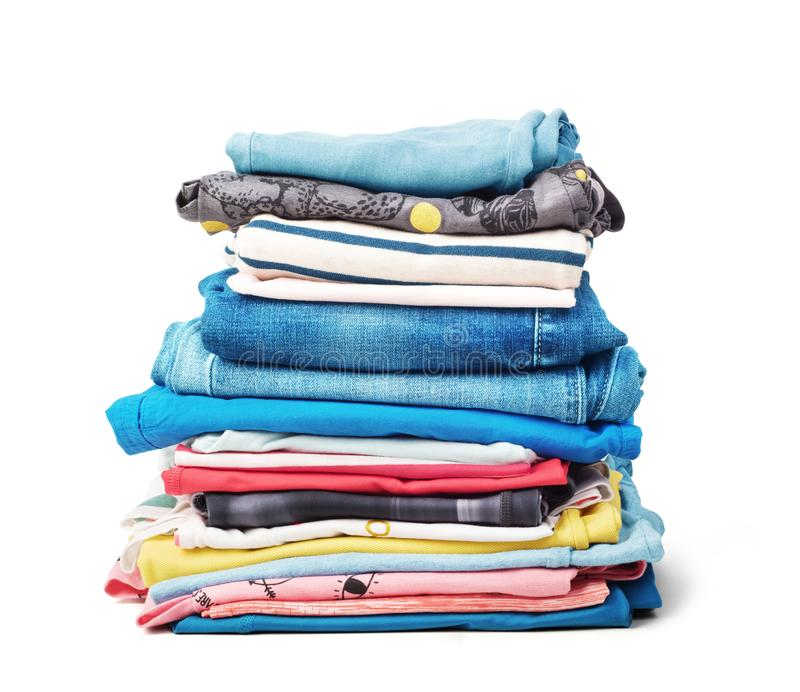
\includegraphics[width=\textwidth]{images/stack.png}
            \vfill
        \end{column}
    \end{columns}
\end{frame}
\begin{frame}
    \frametitle{The Heap}
    \begin{columns}
        \begin{column}{0.5\textwidth}
            \begin{itemize}
                \item Slower to store and retrieve data
                \item Need not know the size of the data
                \item Able to resize, copy, and clone on the fly
            \end{itemize}
        \end{column}
        \begin{column}{0.5\textwidth}
            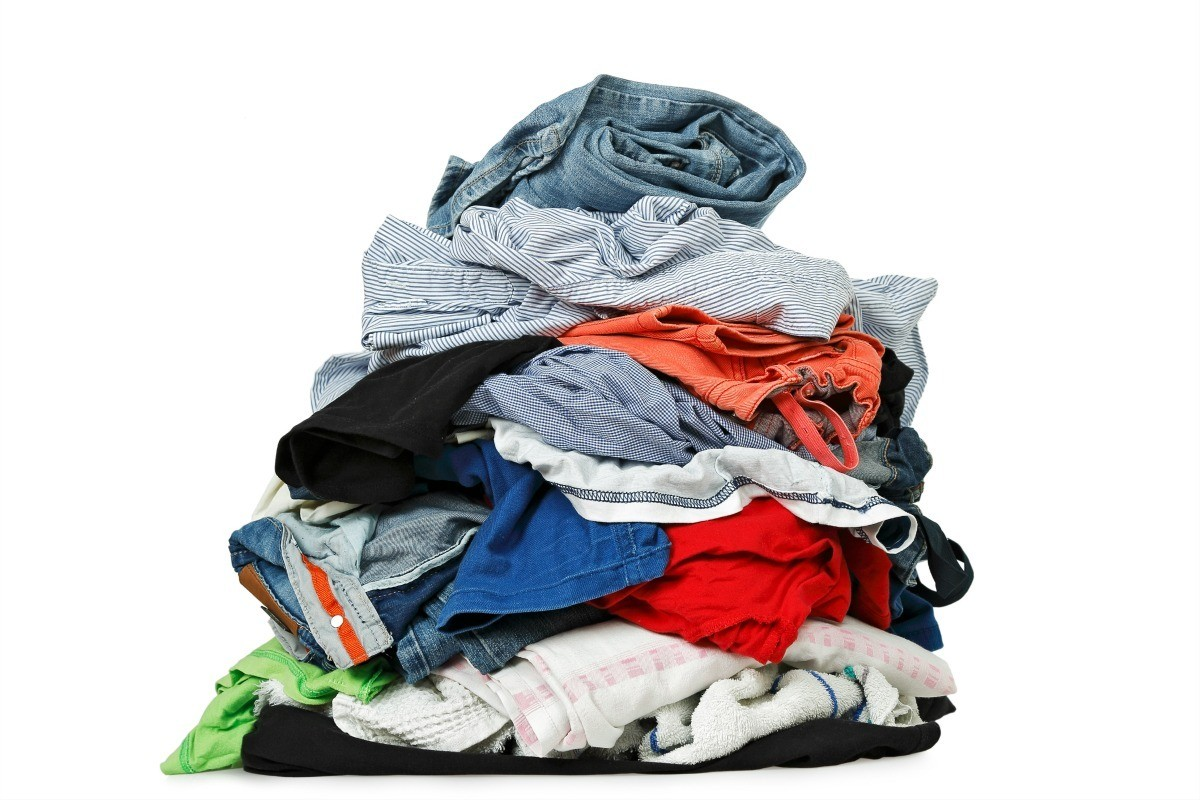
\includegraphics[width=\textwidth]{images/heap.png}
            \vfill
        \end{column}
    \end{columns}
\end{frame}
\begin{frame}[fragile]
    \frametitle{Memory}
    \begin{columns}
        \begin{column}{0.5\textwidth}
            \begin{tabular}{ |c|c| } 
                \hline
                address & value \\
                \hline \hline
                ... & ... \\ \hline
                \verb|0x7fffac86e908| & \verb|00000000| \\ \hline
                \verb|0x7fffac86e909| & \verb|00000000| \\ \hline
                \verb|0x7fffac86e90a| & \verb|00000111| \\ \hline
                \verb|0x7fffac86e90b| & \verb|11100111| \\ \hline
                ... & ... \\ \hline
            \end{tabular}
        \end{column}
        \begin{column}{0.5\textwidth}
            \verb|let x: u32 = 2023;|
            \verb|println!("x addr: {:p}", &x);|
            \verb|// x addr: 0x7fffac86e908|
        \end{column}
    \end{columns}
\end{frame}

\section{Variables and scope}
\begin{frame}[fragile]
    \frametitle{Variable scope}
    \begin{verbatim}
fn main() {
    {
        let x: i32 = 5;
        println!("x = {}", x);
    }
    println!("x = {}", x);
}
    \end{verbatim}
    \hrule
    \begin{verbatim}
error[E0425]: cannot find value `x` in this scope
 --> src/main.rs:6:24
  |
6 |     println!("x = {}", x);
  |                        ^ not found in this scope
    \end{verbatim}
\end{frame}

\section{References}
\begin{frame}[fragile]
    \frametitle{References}
    \begin{itemize}
        \item A reference is the memory address of a value's first byte
        \item Also known as pointers because they \textit{point} to where the data is located
    \end{itemize}
\end{frame}
\begin{frame}[fragile]
    \frametitle{Dereferencing}
    \begin{columns}
        \begin{column}{0.5\textwidth}
        \begin{verbatim}
fn main() {
    let x: i32 = 5;
    let xp: &i32 = &x;
    println!("x = {}", *xp);
    println!("x = {}", xp);
}
        \end{verbatim}
        \end{column}
        \begin{column}{0.5\textwidth}
            \begin{itemize}
                    \item References can be dereferenced to retrieve the original value by using \textit{*}
                    \item Dereferences are usually implicit
            \end{itemize}

        \end{column}
    \end{columns}
\end{frame}
\begin{frame}[fragile]
    \frametitle{Mutable references}
    \begin{columns}
        \begin{column}{0.5\textwidth}
            \begin{itemize}
                \item Variables and references are immutable by default
                \item Mutable variables and references are defined with \textit{mut}
            \end{itemize}
        \end{column}
        \begin{column}{0.5\textwidth}
            \begin{verbatim}
let mut x: i32 = 5;
let xp: &mut i32 = &mut x;
*xp += 1;
            \end{verbatim}
        \end{column}
    \end{columns}
\end{frame}
\begin{frame}
    \frametitle{The Borrow Checker}
    \begin{enumerate}
        \item Data has one owner
        \item Data can have multiple readers, or one writer
    \end{enumerate}
\end{frame}

\section{Safety}
\begin{frame}
    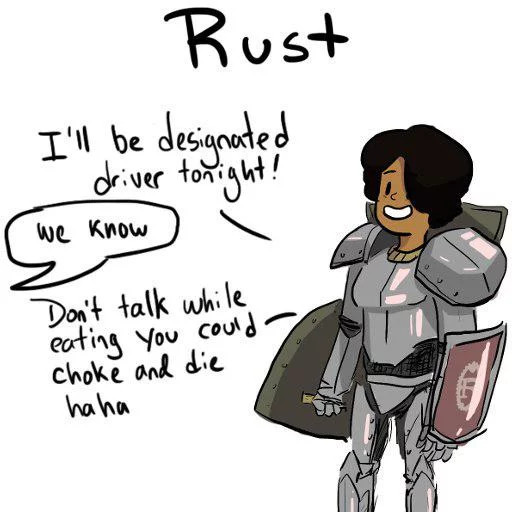
\includegraphics[scale=0.4]{images/rust-taxi.jpg}
    \centering
\end{frame}

\end{document}

